%!TEX root = /Users/markelikalderon/Documents/Git/timaeus/timaeus.tex

\chapter{The Bonds of Life} % (fold)
\label{cha:the_bonds_of_life}

\section{The Soul--Body Union for Mortals} % (fold)
\label{sec:the_soul_body_union_in_mortals}

The previous chapter began making the case for the philosophical significance of Timaean anatomy. We saw, for example, on how understanding the physiology of the liver contributes to our understanding of listening with delight when rationally attending to the \emph{harmonia} of \emph{mousikē}. In this chapter we shall see how the details of Timaean anatomy are relevant to the philosophy of perception in a more general way as well. Perception is an environmental power. It is only possessed by sensible living beings embodied and embedded in an environment and only ever exercised on aspects of that environment. As an environmental power, it is exercised with a corporeal instrument. Perception is a power of the soul exercised through the body. The nature of the soul-body union bears upon how the soul may make use of the body as an instrument. The souls of mortal beings, Timaeus tells us, are bound to the divided marrow within. So in order to learn about the soul-body union in mortal beings, we must learn about the nature of the marrow to which it is anchored.

The soul-body union for mortals differs from the union of the World Soul and the body of the Cosmos. Mortal beings are not only embodied but embedded in an environment. The Cosmos may be an embodied living being, but it is not embedded in an environment---it is the environment. This is related to a further difference. Whereas the World Soul encompasses the body of the Cosmos, the bodies of mortal beings encompasses their soul. The souls of mortal beings are bound to their body and this bond must be protected from the effects of strong powers in the environment. Specifically, the soul is bound to marrow, and this marrow is surrounded by hard bone to protect these bonds from any external impact. Thus the skull is the primary fortification of the sovereign acropolis. Thus the Young Gods, when weaving the immortal and mortal parts together, position these bonds within. In this manner, the body encompasses the soul of a mortal being. By contrast, the Cosmos, though embodied, is not embedded in an environment. Thus there are no strong powers external to the Cosmos that may age or weaken it. And hence no need of corporeal encompassment to protect the interweaving of the World Soul and the body of the Cosmos. So the World Soul may, instead, safely encompass the body of the Cosmos. The souls of mortal beings are bound within since mortal beings are embodied and embedded in an environment with strong powers.

Two features of mortal anatomy are relevant to the soul-body union, the marrow and the bone that encases it. The marrow is not the bond of the soul but that to which the soul is bound. It has the character that it has just for this purpose. So Timaeus' account of the marrow will be informative about the soul-body union for mortals. The bone that encases the marrow is to protect the bond from the effects of strong powers in the environment. The soul of mortal beings has an immortal part and a mortal part. The immortal soul is bound to the marrow in the skull, called the ``brain''. The Young Gods made the skull spherical, in imitation of the shape of the Cosmos and the circular activity of cognition. The mortal soul is bound to marrow as well. Its roots are in the marrow of the spine. When contrasted with the circular skull, we are perhaps struck first by the linear character of the spine. But if we recall that the spine encompasses the marrow that it contains, we recognize that the spine is, more specifically, cylindrical. Recall that motions are either circular or linear. The skull takes its shape from the circular motion of cognition. The spine combines the circular and the linear in its shape. What may we infer about the mortal soul's bond with the marrow of the spine?

The linear aspect of its cylindrical shape is explicable given our previous discussion. Setting aside the possibility of cosmic perception (Proclus, \emph{In Timaeum} 2 83.3–85.31, \citealt{Diehl:1903re}, discussed in chapter~\ref{sec:knowledge_and_opinion}), \emph{aisthēsis} is a power of the mortal soul. \emph{Aisthēsis} involves a corporeal instrument that receives affections from strong powers in the perceiver's environment. Timaeus describes the action of these strong powers as linear. \emph{Aisthēsis} does not merely involve the reception of an affection from without, but importantly, it is the cognizance of the power of the agent that caused that affection. Perhaps the circular aspect of the spine's cylindrical shape reflects the circular activity that constitutes the soul's cognizance of the object of \emph{aisthēsis}. Later Platonists (such as Priscian, \emph{Metaphrasis in Theoprastum}, and Pseudo-Simplicius, \emph{In de anima}) will explicitly characterize perceptual apprehension as circular activity.

% section the_soul_body_union_in_mortals (end)

\section{Marrow} % (fold)
\label{sec:marrow}

God generated marrow from the finest elemental triangles. He chose only those elemental triangles that were unwarped and smooth. The triangles, here, could not be the triangles of planar geometry \citep[293 n2]{Cornford:1935fk}. A warped triangle is not a planar figure. We have encountered this kind of issue before (chapter~\ref{sec:the_circles_of_the_same_and_the_different}). Thus, for example, the Demiurge formed two lines from the soul mixture and bent them back to form two circles. But a geometrical line cannot become a circle. The triangles should be understood on a material model. They are, after all, composed of sensible powers, traces of the Forms in the Receptacle, upon which the Demiurge has imposed form and number. In choosing only the finest elemental triangles, God ensures that they could exactly compose the purest fire, water, air, and earth. (I am uncertain why Timaeus departs, here, from the more usual ordering of fire, air, water, and earth.) God separated these triangles into kinds (presumably their shape) and mixed them in proportions that Timaeus does not reveal (perhaps for fear of impiety). He then fashioned the marrow from this mixture which Timaeus describes as the seed of all mortal kind. 

It is unclear what Timaeus means by this last remark. It is worth pausing over since talk of seeds and associated agrarian imagery predominates in Timaeus' account of marrow. It would be good to know in what sense marrow is a seed since Timaeus goes on to describe marrow as field that receives a divine seed. So is the marrow a seed or a seed bed? And in what sense or senses?

Later (91b1) Timaeus claims that marrow is the source of semen. So the marrow is the seed of all mortal kind since it is at the very least the source of the semen from which subsequent generations of mortals will spring. Notice, as well, the generality of Timaeus. Marrow is not merely the seed of human kind \citep[73]{Waterfield:2008lx} but of mortal kind. This encourages \citet[295]{Cornford:1935fk} to claim that ``the marrow is the fundamental life-substance in all animals and the same substance in all''. As we shall see, that marrow is described as universal seed since it is the fount of semen in mortals is not inconsistent with Timaeus subsequently describing marrow as a field or seed bed.

Though Timaeus speaks of the God in the singular here, the generation of the marrow is clearly a task that the Demiurge assigned to the Young Gods. The Young Gods, in generating the mortal parts, imitate the Demiurge's generation of the immortal part. Here, particulary, the \emph{mimēsis} is striking. The Demiurge generates the immortal soul by taking indivisible and divisible Being, Sameness, and Difference, mixing these, and using this mixture to fashion the immortal soul. Similarly, God generates marrow by selecting its components, mixing them, and fashioning the marrow. God's procedure is the corporeal analogue of the Demiurge's generation of the incorporeal soul.

God implanted in the marrow various kinds of soul. Allow me to make two sets of remarks about this deceptively simple claim.

First, \emph{phuteuō} can mean implant, beget or engender, or to produce or bring about more generally. I translate (with \citealt[271]{Archer-Hind:1888qd}, \citealt[293]{Cornford:1935fk}, \citealt[70]{Lee:2008ca}, \citealt[77]{Taylor:1929ov} \citealt[73]{Waterfield:2003gs}, and \citealt[67]{Zeyl:2000cs}) \emph{phuteuōn} as implanted. Even if \emph{phuteuōn} could mean engendered in this context (as \citealt[191--3]{Bury:1929jb} translates), given the prominence of the agrarian imagery, the association of implanting carried by the Greek is salient. Recall that the immortal soul, in its celestial descent was sown in the instruments of time, and this signaled a greater involvement in corporeality than when it was merely a passenger in a stellar vehicle (chapter~\ref{sec:the_laws_of_destiny}). When it is implanted in the marrow that involvement is greater still for it is now embodied and embedded in an environment with strong powers.

Second, God implants in the marrow various kinds of soul. What kinds of soul does Timaeus have in mind? There are two alternatives. The kinds in question may simply be the immortal and mortal kinds. Or, given that the mortal soul has spirited and appetitive parts, the kinds may be reason, spirit, and appetite. On the first alternative there are two kinds on the second there are three. This may not seem like much of a difference given that the second kind of the first alternative, the mortal soul, divides exhaustively into the second and third kinds of the second alternative, spirit and appetite. But indifference between these alternatives betrays an insensitivity to a substantive explanatory difference. Are there two fundamentally different kinds of soul or three? Cast in these terms, it would seem that there are two, the immortal and mortal kind. The former does not perish upon death though the later does (though later Platonists envision the possibility of life after death for even the mortal soul, to animate the powers of shades in Hades, say). The Demiurge generates the immortal soul. The Young Gods generate the mortal soul. For recall, the Demiurge is incapable of generating anything mortal. And while spirit and appetite differ in their powers, locations and corporeal instruments, there does not seem to be a fundamental difference between them the way there is between sovereign reason and the broader \emph{polis}. This was manifest in the political toplogy of the soul. Reason occupies the acropolis, raised on a hill, surrounded by water and joined to the mainland and the broader \emph{polis} by a narrow isthmus. The social distance between the occupants of the acropolis and the occupants of the broader \emph{polis} is manifest in their spatial distance. And the splendor and fortification of the acropolis emphasize this. 

Having implanted the various kinds of soul in the marrow, God now divides that marrow. The divisions of the marrow correspond to the number and shape of the kinds of the souls implanted there. Again, this is a deceptively simple claim.

First, note the oddity of God's procedure. The kinds of soul are first implanted in the marrow and then the marrow is separated and formed into shapes that match the kinds. One might have expected, instead, that the marrow was divided and shaped first and then the various kinds of souls implanted in the appropriately shaped divisions of marrow. Why does God proceed otherwise? Given His understanding and benevolence, it must be for the best. Perhaps God implants the various kinds of soul in undivided marrow because of the unity of the souls of mortal beings. It is one thing for Timaeus to distinguish parts of the soul. It is another to maintain that there are distinct rational, spirited, and appetitive souls. Even reason persisting when spirit and appetite perish, does not, by itself, establish this. Perhaps, then, God's implanting soul in undivided marrow dramatically emphasizes the unity of the soul of mortal beings (though, of course, questions remain).

Second, the number and kinds of shapes of the divided marrow correspond with the number and kinds of shapes of the souls implanted there. What is the number of souls? If the number of souls is one in each case there is not much point in making number explicit. This really only makes sense if the number of a kind of soul could be more than one. So, for example, we know that there is only one part of the soul implanted in the head, the immortal part. What about the mortal part? The mortal part itself divides into spirit and appetite. if there are separate divisions of marrow for spirit and appetite, then the number in each case is one. But that is the trivial case. But if the mortal soul is implanted in its own marrow, then the number of souls (strictly parts of soul) implanted there are two. Thus the fundamental division of the soul into the immortal and mortal part is preserved, consistent with the further subdivision of the mortal soul required for tripartition.

Third, Timaeus' language here remains neutral concerning an important topic. What is the relationship between the shape of the marrow and the shape of the soul implanted there? If the soul is extended, then perhaps the marrow must be so shaped otherwise the soul would not fit. Or, if the soul is inextended, perhaps the shape of the marrow is modeled on an inextended paradigm. Timaeus does not specify the explanatory relationship, such as efficient or paradigmatic causation, if any, between the shape of the marrow and the shape of the soul implanted in it. Timaeus merely claims that they match.

God first divides the marrow that receives the immortal soul. This He makes into a voluminous sphere. Since the sphere of marrow received the immortal soul, and given its divine nature, Timaeus likens the marrow to a field receiving divine seed. God calls this sphere of marrow ``brain'' (\emph{engkephalon}).

First, while Timaeus remains silent on the explanatory relationship between the shape of the soul and the shape of the marrow, details of the narrative would seem to rule out one natural alternative. Notice that the kind of soul---strictly, a part of a unified soul---is implanted in the undivided marrow. The marrow is then divided. And only then is it shaped into a sphere. That means that the immortal soul was implanted in the marrow before it was spherical. If that is right, then it is not the case that the marrow has its shape so that the relevant kind of soul will fit. The immortal soul fit fine when implanted in the undivided marrow.

Second, the agrarian imagery continues. The soul, and not the marrow, is now portrayed as a divine seed. The immortal soul is divine. It can apprehend in understanding divine intelligible things, and so assimilate to them. Timaeus has already described the soul as sown in the instruments of time and subsequently implanted in divided marrow. Since seeds are what one plants, this is a natural elaboration of the earlier agrarian imagery. But it is an elaboration. Timaeus highlights the way in which seeds contain within themselves the power of growth and vital activity. Perhaps, the immortal soul is the divine seed since it is a divine principle of vital activity implanted within corporeal material designed to receive it. The marrow, of course, in being generated from the finest elemental triangles in the right proportions, was prepared to receive the divine seed and so is likened to a field.

Describing the soul as divine seed implanted in the field of marrow is consistent with Timaeus' earlier description of marrow as universal seed. Indeed, the descriptions may be complementary. The marrow is like a field since it receives the divine seed and this activates vital activity in the newly incarnate mortal. The marrow is itself universal seed since it is the fount of semen. But as this is vital activity, the marrow is only the fount of semen insofar as the divine seed has been implanted there by God.

Third, a name is bestowed upon this spherical division of marrow. God calls it ``brain''  (\emph{engkephalon}). As \citet[77 n2]{Taylor:1929ov} and \citet[293 n3]{Cornford:1935fk} observe, this is most likely derived from \emph{en kephalē}, in the head. Given its gross observable features, it is perhaps natural to first regard the brain as the marrow of the skull. Timaeus claims that every living thing has the head as the container for the brain.

If the immortal soul is assigned to one division of marrow, the mortal soul is assigned to a plurality of divisions of marrow. God forms these into shapes that were both circular and linear. They have cylindrical shapes. Think, for example, of the shape of the marrow in the femur, or a bone in a finger. Upon these God bestowed the name ``marrow''.

The marrow is a divided seed bed. Nevertheless, from these, as from anchors, God bound the whole soul.

First, concerning the plural reference of ``these'', I take Timaeus to mean not only what God calls ``marrow'' but also what God calls ``brain''. For what is bound is the whole soul. And the whole soul includes the immortal part implanted in the brain.

Second, Timaeus shifts from agrarian to nautical imagery. The divided marrow anchors the whole soul. If the marrow is an anchor, then the soul is a ship tethered to this anchor by ropes or chains. The buoyancy of a ship keeps it afloat and so up from the floor of the sea. The image suggests that the corporeal is weighing down the whole soul which, if left to its own devices, might move upward in a celestial ascent (as in the \emph{Phaedrus} myth).

Third, Timaeus is unfortunately reticent about the nature of the bonds that anchor the whole soul to the divided marrow. Whatever their nature, they must be so as to bind the incorporeal to the corporeal. If we think of corporeal bonds such as ropes and chains this can seem puzzling. But not all bonds are corporeal. Timaeus, for example, claims that proportion is a bond, but proportion is not a body. Moreover, we have seen how this incorporeal bond may bind the corporeal. The Empedoclean ``roots'' are bound together by proportion in the body of the Cosmos. Timaeus does not say that the bonds that anchor the whole soul in the divided marrow are proportions. Nevertheless, what reflection on proportions as bonds reveals is that there is room within Timaeus' framework for a bond that binds the corporeal and the incorporeal.

We are now in a position to observe that Timaeus has posited three kinds of bonds, with the bonds that anchor the whole soul to the divided marrow being an intermediary kind. Let us consider the extremes first. On one extreme, there are incorporeal bonds that can only be undone by the agent that bound them. Examples of these are the proportional bonds that bind the primary bodies of the Cosmos  (32c3--5, chapter~\ref{sec:the_elemental_composition_of_the_corporeal}), the Young Gods (41a7--b6, chapter~\ref{sec:the_demiurge_addressing_the_gods}), the immortal part of the soul (43d, chapter~\ref{sec:the_shock_of_embodiment}), and the opposed extremes of white and black (68c7–d7, chapter~\ref{sec:the_eyes}). On the other extreme, there are corporeal bonds that can be undone even by agents other than the one that bound them. The invisible rivets with which the Young Gods bind the mortal parts (43a3–6, chapter~\ref{sec:the_shock_of_embodiment}) is an example of this. The bonds that anchor the whole soul to the divided marrow seem to be an intermediary bond that shares features with each of the opposed extremes. While the bonds that anchor the soul are most likely incorporeal, like corporeal bonds, they may be undone by agents other than the one who bound them, thus making the fortification of the acropolis necessary.

% section marrow (end)

\section{Bone} % (fold)
\label{sec:bone}

The whole soul is anchored to the divided marrow. And around this God constructed a shelter from a framework of bone. Bone is the primary fortification of the acropolis, the walls that safekeep its sovereign occupants.

Timaeus begins by describing the generation of bone. He evidently takes his lead from Empedocles but offers a modification of that account. According to Empedocles:
\begin{verse}
	And pleasant earth in her well-built channels (\emph{choanoisi})\\
	received two parts of gleaming Nestis out of eight\\
	and four of Hephaistos; and they become white bones\\
	fitted together with the divine glues of harmony.\\
	(Empedocles, DK 31B96; \citealt[62 245]{Inwood:2001ve})
\end{verse}
Nestis is a Sicilian water goddess, and Hephaistos is associated with fire. Thus on a straightforward reading of the fragment, bone is generated by combining four parts fire with two parts earth and two parts water. (Though some commentators take Nestis to refer to water and air, perhaps under the influence of the general conviction that all four ``roots'' are present in every compound body, \citealt[209 n2]{Wright:1981zr}.) 

\citet[301-2]{Palmer:2009qf} maintains, however, that the straightforward reading of the fragment is flat footed. Specifically, he maintains that \emph{choanoisi} should not be translated as channels or hollows (as \citealt[151 n1]{Guthrie:1965ys}, \citealt[208--9]{Wright:1981zr}, \citealt[62 245]{Inwood:2001ve} do), but rather as a crucible. Hephaistos' involvement in the fragment makes this reading salient. So understood, Empedocles is not merely putting forward a list of ingredients from which bones may be mixed but a recipe for the generation of bone. Specifically, earth is first transformed into mud with the addition of water, and then this mixture is hardened by being fired in the crucible.

Timaeus would seem to accept a similar interpretation, for his account of the generation of bone further elaborates upon the metallurgic imagery. Moreover, Timaeus is similarly offering a recipe, a description of the process by which bone is generated. At the very least, Timaeus seems to regard this kind of interpretation as independently defensible, regardless of whether Empedocles actually subscribes to it. Perhaps this licenses the departures Timaeus makes from Empedocles' account. 

According to Timaeus, the procedure for generating bone consists of three steps:
\begin{enumerate}[(1)]
	\item God selects only earth that is smooth and pure by filtering it
	\item God mixes the selected earth with marrow
	\item God places the compound first in fire and then water, repeatedly
\end{enumerate}
Let us consider these in turn.

(1) \emph{God selects only earth that is smooth and pure by filtering it}. There is precedent for this in God's selection of the triangles that compose marrow. Only the finest triangles, unwarped and smooth, were chosen. Concerning the material that will fortify the acropolis, God is similarly selective. However, He begins not with elemental triangles, but with the primary body, earth. This perhaps explains the difference between the criteria for selection. Earth may be smooth, like the triangles that compose marrow, but no mention is made about being unwarped. The relevant sense of unwarped, I take it, is applicable to the elemental triangles and not to the bodies that may be composed of such triangles. Presumably the smoothness of earth consists in the cubes that compose it being small and relatively uniform in size. God selects only the finest earth. Not only is God selecting for the smoothness of earth but also its purity. So any other primary bodies, such as air or water, are filtered out and perhaps any unattached elemental triangles as well. The selection is described as a kind of filtering or sifting, and so we may imagine the craftsman God filtering earth through a sieve that selects only sufficiently small cubes of earth.

(2) \emph{God mixes the selected earth with marrow}. The first step was an elaboration of the Empeoclean account insofar as Empedocles makes no mention of the divine selection of earth. If the first step of the procedure is, in this way, an elaboration, the second step is a more significant departure. According to Empedocles, earth and water are mixed and so form the substantial mixture from which bone is generated. This is true both on Palmer's \citeyearpar{Palmer:2009qf} interpretation and the more straightforward alternative. The only difference is that, on the latter, more besides goes into the substantial mixture. However, on Timaeus' account, water is no part of the substantial mixture but is used, instead, to treat that mixture in the process of bone generation. Timaeus substitutes a secondary body, marrow, for this primary body, water, to mix with earth. However, marrow is understood to be moist in the way that water is. And so presumably the resulting compound is muddy if not strictly speaking mud.

Why substitute marrow for water? Timaeus does no explicitly say. Consider, however, the following two suggestions.

First, perhaps we are meant to imagine that the result of this procedure is a compound of bone and marrow, with hard bone on the outside and soft marrow within. Perhaps the moist marrow is dusted with earth that binds to it. Repeatedly firing and watering the compound results in soft marrow surround by hard bone. I have my doubts. First, we depart from Empedocles where, on any interpretation, earth is mixed with water. If the Empedoclean parallel is to be maintained, then earth would be mixed with moist marrow. But it is not. On the present suggestion, earth merely dusts the moist outer surface of the marrow and binds to it. Another problem concerns the further fabrication that bone undergoes. Thus God fabricates the spherical skull on a lathe---a hazardous procedure, if the marrow remains within.

For these reasons I favor the second, admittedly speculative, suggestion. Perhaps generating bone from a substantial mixture that includes marrow guarantees that bone has some affinity for marrow. If so, that only raises the further question, why should the fortification of the acropolis share an affinity with its occupant? Consider the following reason available to Timaeus. Bone must be hard in order to protect the the divine bonds of life anchoring the whole soul to the divided marrow within from external impact. Perhaps bone, in being composed, in part, of marrow, retains an affinity with marrow and this functions to lesson the effect of any external impact upon the marrow. Thus when an external blow impacts upon the head, the hardness of the skull may prevent the marrow from being directly impacted, but the marrow will move within that hard skull and suffer a secondary impact against it. But suppose the skull, though hard, has an affinity with marrow. This would mean that it is less likely for the skull to act upon the marrow upon the secondary impact. After all, like does not act upon like. Having marrow as part of the substantial mixture of bone would thus function analogously to padding within a helmet (see figure~\ref{fig:helmet}).

\begin{figure}[htbp]
	\centering
		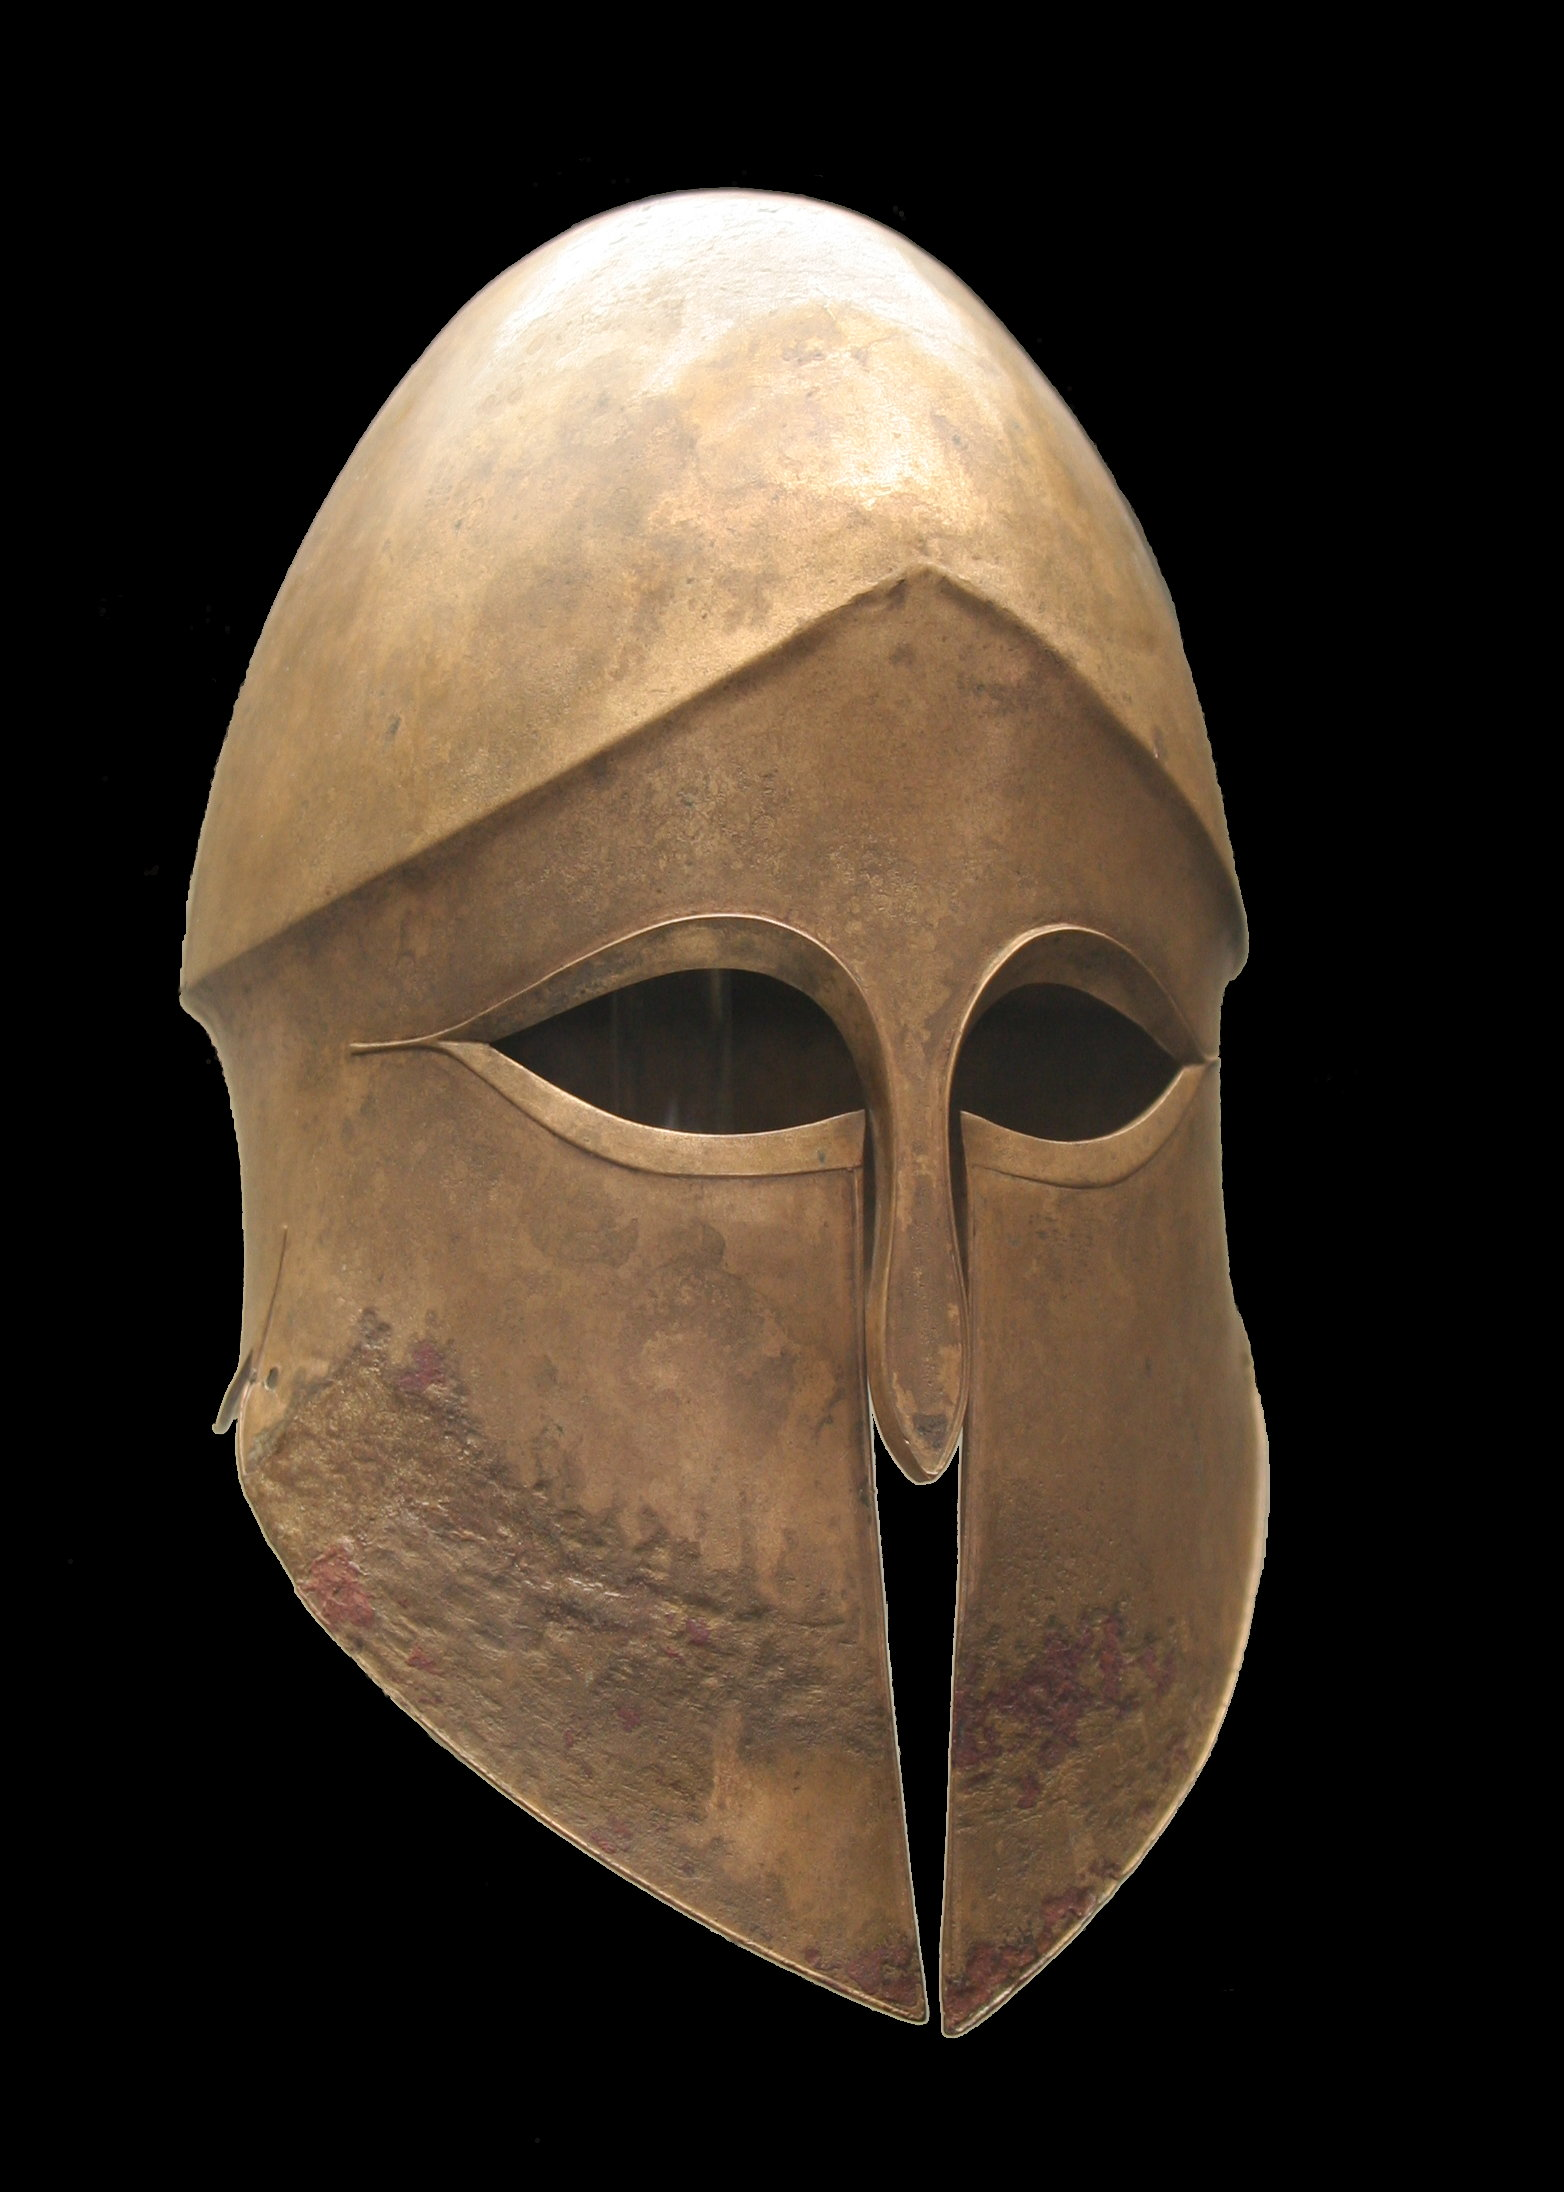
\includegraphics[scale=0.1]{graphics/helmet.jpg}
	\caption{Bronze Corinthian helmet, ca 500 BCE, Staatliche Antikensammlungen}
	\label{fig:helmet}
\end{figure}

(3) \emph{God places the compound first in fire and then water, repeatedly}. We have already observed that Timaeus replaces water with marrow in the substantial mixture from which bone is generated. Water plays a role in the procedure for generating bone but not as a part of the substantial mixture. Instead, Timaeus assigns to water a distinct role in his further elaboration of the metallurgic imagery. God takes the compound, the substantial mixture of earth and marrow, and fires it. He then cools it by plunging the compound in water. These two steps, firing and watering, are repeated many times. The metallurgic imagery here is vivid, especially if we bear in mind Hephaistos' involvement in the Empedoclean account. We are clearly meant to imagine a blacksmith pulling metal out of the fire of the forge and cooling it by plunging it into water. 

Nevertheless, Timaeus' rationale for this procedure is not metallurgic, at least not in the first instance. God exposes the compound to fire and water so that it may not be soluble by either primary body. Notice that there is no explicit mention here of hardening. Though since we began with a muddy mixture of fine earth and moist marrow, a soft compound, unlike the hard bone that is generated from repeatedly firing and watering it, it is safe to say that that the compound is also hardened in this process. The metallurgic imagery encourages this. And it is appropriate that hard bone be produced in a divine forge, like Hephaistos', since it is the fortification of the marrow, and among the things forged by a blacksmith is, importantly, armor. That the repeated firing and watering not only makes the substantial mixture insoluble by either primary body but also hardens it is later explicitly confirmed in Timaeus' discussion of sinews (74b). There he claims that increasing the number of firings and waterings increases the hardness and inflexibility of bone.

The procedure for the generation of bone results in boney stuff from which bones are themselves fabricated. The relevant craft seems to shift from metallurgy to carpentry. Thus, for example, the craftsman God seems to fabricate the skull on a lathe. Timaeus describes the fabrication of the skull and the vertebrae that compose the spine. These are not the only bones recognized by Timaeus. Timaeus singles out these two classes of bones given their special status. All bones contain marrow. And all marrow contains soul. But not all marrow contains enough soul for intelligence. The skull contains sufficient marrow to be the seat of intelligence. If the immortal part of the soul is anchored to the marrow of the skull, then the mortal part of the soul is anchored, primarily, to the marrow in the spine.

The spherical skull is fabricated by spinning it. Clearly the craftsman God fashioned the spherical skull on a lathe. It is unclear, though, how the spherical skull comes to encompass the brain. The alternative reading, where marrow is not part of the substantial mixture from which bone is formed but is rather dusted with earth that binds to it, admittedly faces no such difficult. It has the advantage that the soft marrow is baked in, and only the earth-dusted surface is hardened into bone around it. This is a neat solution to our present difficulty. But, again, it fails to parallel Empedocles in not making marrow a part of the substantial mixture, and it is hard to square with fashioning the skull on a lathe, which would be a procedure fraught with danger if possible at all.

After fabricating the skull, God fabricates the vertebrae that compose the spine. Like the skull, vertebrae are composed of hard bone and encompass marrow that anchors a great amount of soul. There are, however, a number of striking contrasts:
\begin{enumerate}[(1)]
	\item While the skull is one, the vertebrae that compose the spine are many
	\item While the skull is circular, the spine is linear, the vertebrae that compose the spine being vertically stacked
	\item While the skull is inflexible, the spine is flexible since there are pivots between the vertebrae.
\end{enumerate}
Let us consider these differences in turn.

(1) \emph{While the skull is one, the vertebrae that compose the spine are many}. This may be a corporeal echo of the structure of the soul. Recall, the Circle of the Same is sovereign in that it governs the revolution of the Circle of the Different. And since it is sovereign, the Demiurge allows it to remain undivided unlike the Circle of the Different. The skull is the primary fortification of the acropolis in which the immortal soul is anchored. The immortal soul has sovereignty over the mortal soul and the body that it animates. Presumably for this reason, its primary fortification consists in the unitary skull. The mortal soul, by contrast, is anchored in the spine. As it is governed, like the Circle of the Different, it is not exempt from division.

(2) \emph{While the skull is circular, the spine is linear, the vertebrae that compose the spine being vertically stacked}. The skull is a sphere made in imitation of the shape of the Cosmos. The spine, however, is linear, being composed of vertically stacked vertebrae. This is a corporeal manifestation of a difference in cognitive power, broadly conceived. Whereas the immortal soul anchored in the brain encased within the skull engages in the circular activity of cognition, the mortal soul, anchored in the marrow of the spine is subject to linear \emph{aisthēsis}. \emph{Aisthēsis} is a power of the mortal soul that involves a corporeal instrument that receives affections from strong powers in the perceiver’s environment. And Timaeus describes the action of these strong powers as linear. Thus the fortification of the marrow that anchors the mortal soul reflects, in its shape, the power of \emph{aisthēsis}, just as the fortification of the acropolis reflects, in its shape, the power of cognition.

While the spine is linear, it encompasses the marrow within its stony substance. So, as we observed before, its overall shape is that of a cylinder. The linear aspect of the cylinder may reflect the linear nature of \emph{aisthēsis}, but its circular aspect may reflect the power to apprehend the objects of \emph{aisthēsis}.

(3) \emph{While the skull is inflexible, the spine is flexible since there are pivots between the vertebrae.} This third difference is related to the first. The spine is compound, being composed of a plurality of rigid parts, the individual vertebrae, joined together with pivots. Given its plurality and the nature of its construction, the spine, as a whole, is flexible in the way that the skull, as a whole, is not. And again this may be a corporeal echo of the structure of the soul. Compare how the divisions in the Circle of the Different in the World Soul is manifest and make possible the complex motions of the wanderers. Similarly the divisions in the spine is manifest and makes possible the flexible movement of the spine. 

% section bone (end)


\section{The Location of the Mortal Soul} % (fold)
\label{sec:the_location_of_the_mortal_soul}

The mortal soul is located below the neck in the thorax. The spirited part of the mortal soul is specifically located in the the upper thorax above the midriff or diaphragm. The appetitive part of the mortal soul is, by contrast, in the lower thorax between the midriff and the navel. So the mortal soul and its parts are associated with definite corporeal regions. How does this cohere with the mortal soul being anchored to the marrow within the spine? Is the mortal soul enclosed within the spine? Or does it extend into the broader region of the thorax?

Comparing the soul-body union of mortals with that of the Cosmos can encourage the former alternative. On at least one telling of the World Soul's union with the body of the Cosmos, the corporeal is constructed within the World Soul so that it encompasses the body of the Cosmos. By contrast, the soul of mortal beings is portrayed by Timaeus as being encompassed by the body that it animates. Thus, for example, the immortal soul is represented as the sovereign occupant of the acropolis of a \emph{polis}. This very specifically suggests that the immortal soul is within the skull with the marrow it is bound to. But if the immortal soul is bound within the skull, the mortal soul should be bound within the spine. But if it is bound within the spine, then it does not extend into the broader region of the thorax.

Perhaps the sense in which soul is located within bone and the sense in which it is located without, in broader regions of the body, differ. 

If we take seriously the idea that the immortal soul is the sovereign occupant of the acropolis, then it is located within the skull, bound to the brain. If the mortal soul is parallel, the it is located within the spine bound to its marrow. This is really the only way to make sense of the fortifying role of bone, its protecting the bonds that anchor soul from external impact. If that is right, then the mortal soul must be located in the broader region of the thorax in another sense. But what sense is that?

First, it is important to understand that the powers of the mortal soul are environmental powers. At the very least, they are powers of sensible living beings embodied and embedded within an environment. And many of these powers, such as perception, are only ever exercised on aspects of that environment. Moreover, environmental powers have corporeal instruments by which they act. Perhaps the mortal soul is located in the broader region of the thorax in the sense that the corporeal instruments of its powers are located there. Indeed, this seems to be just what Timaeus was describing in his description of the primary and secondary organs of the spirited and appetitive parts of the mortal soul (discussed in chapter~\ref{cha:the_flesh_and_the_mortal_soul}).

But a question remains. How does soul, anchored to marrow within, animate corporeal instruments without? Perhaps the illuminationist imagery that Proclus discerns in the ensoulment of the body of the Cosmos is relevant (discussed in chapter~\ref{sec:the_embodiment_of_the_world_soul}). Soul, having been placed in the center of the Cosmos, illuminates, by its powers, the whole of the Cosmos and beyond (\emph{In Timaeum} 2 108, \citealt{Diehl:1903re}). Perhaps, the soul bound within the marrow of bone animating the corporeal instruments without is understood, in this way, on the model of illumination. On the illuminationist model, the soul is like the Sun. And its powers that animate the body are like the light emitted by the Sun. The Sun does not need to depart from the Heavens to illuminate the Earth below. Similarly, the soul does not need to depart from its boney fortification to animate the surrounding flesh. Just as \emph{nous} illuminating the liver to produce rational imagery was not a physiological claim (all is dark within, and the liver would anyway be in the shadow of the heart and lungs, discussed in chapter~\ref{sec:appetite}), so soul bound to marrow within bone illuminating the flesh without is not itself a physiological claim (again, all is dark within, and bone is anyway opaque). In the present instance, the illuminationist imagery is better understood as making a claim in the metaphysics of psychology. Later Platonists would explicate the metaphorical metaphysics in terms of ever more elaborate schemes of procession and reversion.

% section the_location_of_the_mortal_soul (end)

\section{The Incorporeality of the Mortal Soul} % (fold)
\label{sec:the_incorporeality_of_the_mortal_soul}

Where is the mortal soul located? In a way, it depends upon what is at stake in the answer. Insofar as what is at stake depends on the mortal soul being anchored to marrow encased in bone, that is where it is located. However, insofar as what is at stake depends on the corporeal instruments of the powers of the mortal soul being located in the broader region of the thorax, that is where it is located. Wherever the mortal soul located, given what is at stake in saying so, that the mortal soul is, in fact, located, by itself, does not establish that it is a body. The Greenwich Mean Line is located, but the Greenwich Mean Line is not a body. So from the mortal soul being located we cannot immediately infer that it is corporeal. Again, recall, for Timaeus, extension is not the mark of the corporeal, being sensible is. So what is the corporeal status of the mortal soul?

One obstacle to answering this question is Timaeus' own reticence. Timaeus has described in detail the psychogony of the World Soul and in less detail the psychogony of the immortal soul of mortal beings (though perhaps this is a narrative accommodation of redundancy since the cases are parallel). But Timaeus has not described the Young Gods imitating demiurgic psychogony. Just as the psychogonies of the World Soul and the immortal soul were informative about their natures, so too would an account of the Young Gods' generation of the mortal soul be informative about its nature. Unfortunately, Timaeus simply omits such an episode from his narrative. And so we must look elsewhere for evidence about the corporeal status of the mortal soul. Not only must we look elsewhere for evidence, but the missing psychognony of the mortal must itself be accounted for.

Consider the hypothesis that the mortal soul is corporeal. It would be tempting to identify the parts of the mortal soul with the primary organs associated with them, or perhaps the complex of primary and secondary organs. Thus spirit, on this hypothesis, would be identified with the heart, or perhaps the complex of heart and lungs. And appetite would be identified with the liver, or perhaps the complex of liver, spleen, and oesophagus. One problem with this suggestion is that there are other organs in the thorax that are presumably animated by the mortal soul. Are we then to simply identify the mortal soul with the body that it animates? That seems wrong. The mortal soul is the principle that animates the body and so uses it as an instrument. Moreover given the ethical functions assigned to the primary and secondary organs, given the political topology of the mortal soul, these are unlikely to be the principles that animate the biological functions of the other organs.

Just as there are two ways of understanding the location of the mortal soul, there are two candidates for identifying the mortal soul. Perhaps, instead, the mortal soul is identified with the marrow of the spine. Spirit might specifically be the marrow of the spine that corresponds to the region of the upper thorax, and appetite the marrow of the spine that corresponds to the region of the lower thorax. Other than being the universal seed of mortal life, and so playing a role in the perfection of a truly comprehensive Cosmos, the marrow does not have a specific ethical function that might obscure how it could be a principle of vital activity. And yet, how does a body use another body as an instrument of its power? Perhaps they mechanically interact. The problem is that Timaeus provides no such account of how the marrow pulls the levers of the human body.

Perhaps we need a broader understanding of the corporeal. Perhaps the corporeal is not restricted to bodies, divisible beings, but includes, as well, their motions. Perhaps the mortal soul should not be identified with the human body or its parts but rather with its motion or the motion of its parts. The mortal soul would be corporeal, on this broader understanding, without being identified with a body.

In support of this hypothesis, one might cite Timaeus' claim that the Young Gods construct the mortal soul from the \emph{pathēmata} they are subject to, where these are affections of the body that are liable to give rise to \emph{aisthēsis} in the broad sense that includes perception and sensation, both painful and pleasant, and desire. And earlier Timaeus promised to frame an account of the mortal soul from such affections. Perhaps the account is framed from these in the sense that in the account the mortal soul is framed from such affections. This might suggest that the mortal soul is a kind of vital activity of a body subject to affections from strong powers without.

I suspect that this kind of account is the best available understanding of the corporeality of the mortal soul. Unfortunately, a residual problem remains. If anything, the mortal soul is the principle of vital activity. And if it is, it cannot be identified with that activity. And so even on this broader understanding of the corporeal nature of the mortal soul, where it is not identified with a body, but, rather, with the vital activity of a body, it remains inconsistent with the mortal soul being the principle of the vital activity of its corporeal instruments.

If the mortal soul is not corporeal, then it is incorporeal. But there is a puzzle here as well. The mortal soul is not generated from the soul mixture left over from when the Demiurge generated the immortal soul. That mixture was used up in its apportioning. Nor has Timaeus narrated the Young Gods mixing indivisible and divisible Being, Sameness, and Difference or any other materials---perhaps merely divisible Being, Sameness, and Difference---to generate the mortal soul. We have not been told that the mortal soul is invisible, the way the immortal soul is. (And, recall, the sensible is the mark of the corporeal, chapters~\ref{sec:the_generation_of_the_cosmos} and \ref{sec:the_elemental_composition_of_the_corporeal}.) So what positive reason is there to think that the mortal soul is incorporeal? How are we to solve the case of the missing psychogony?

Perhaps, Timaeus' reticence about the psychogony of the mortal soul is less of a problem than a clue. Why omit such an account? One excellent reason would be because it is simpy unnecessary. One way of understanding how it might be unnecessary bears on the unity of the immortal and mortal souls. Though Timaeus distinguishes the immortal and mortal parts of the soul, there is reason to doubt that there are two, let alone three, separable souls animating the bodies of mortal beings. As we shall see in the next section, understanding the unity of the soul is not unrelated to understanding why a psychogony of the mortal soul is unnecessary and so omitted without loss in Timaeus' narrative.

% section the_incorporeality_of_the_mortal_soul (end)

\section{The Unity of the Soul} % (fold)
\label{sec:the_unity_of_the_soul}

The Demiurge generates the immortal soul form a mixture of indivisible and divisible Being, Sameness, and Difference. The immortal soul thus generated is invisible and incorporeal. Though it has a share of corporeality in the sense that, since it is partly composed of divisible Being, it may be located in space like sensible bodies, and its activities occur in time. As the pscyhogony makes explicit, soul is an ontological intermediary between the intelligible and the sensible. As Philoponus suggests, partly for this reason, being incorporeal is no obstacle to being bound to marrow, specifically to the brain encased within the skull, the primary fortification of the acropolis.

All marrow contains soul. But not all marrow contains sufficient soul for intelligent activity. Only the brain and the marrow of the spine do. But even the marrow with insufficient soul for intelligence is not without soul. But if that is right, then there is a puzzle. Not all of the following could be true:
\begin{enumerate}[(1)]
	\item The soul is exhaustively divided into immortal and mortal parts
	\item The brain wholly contains the immortal part of the soul that is bound to it
	\item The marrow of the spine wholly contains the mortal part of the soul that is bound to it
	\item All marrow contains soul
	\item The brain and the marrow of the spine do not exhaust all the marrow that there is.
\end{enumerate}
Consider the significance of this last claim. For example, there is marrow in the femur, if not enough to contain sufficient soul for intelligence. But if the soul is exhaustively divides into immortal and mortal parts, and the brain and the marrow of the spine contain the whole of these, then there is no soul for the marrow of the femur to contain.

The most economical interpretation that resolves this puzzle claims that there is only one soul. This one soul may be variably bound to divided marrow. Marrow can contain more or less soul by having more or fewer bonds to the one soul. If it has sufficient number of bonds, then the marrow is capable of intelligent activity, understood broadly to include, not just opinion and reasoning, but perception and sensation as well. The skull contains sufficient marrow for the brain to be the seat of cognitive activity. In that sense the brain contains the rational part of the soul. The marrow of the spine, though incapable of opinion and reasoning, is not itself devoid of cognitive activity, broadly understood. If \emph{aisthēsis}, understood as perception and sensation, painful and pleasant, and desire, is a power of the mortal soul, then the corporeal instruments of \emph{aisthēsis} are animated by the soul contained within the spine. 

The number of bonds marrow can sustain to the one soul may makes a difference to the kind of intelligent activity that it can engage in, perhaps with the help of the corporeal instruments that it animates. But if that is right, then both the unity of the soul, and the lack of need for a separate psychogony for the mortal soul are readily explicable.

There is one soul. It was generated by the Demiurge. Since there is one soul and not two, there is no need for a further psychogony since no further soul is generated. What then are the immortal and mortal parts of the soul? Importantly, these parts only get distinguished with the soul's embodiment. 

The brain consists in sufficient marrow to have enough bonds to the one soul that it may engage in cognitive activity such as understanding, knowledge, opinion, and reasoning. Opinion may depend upon \emph{aisthēsis}, which in turn depends upon corporeal instruments to receive the affections of strong powers in the environment, but understanding, knowledge, and reasoning do not seem to have corporeal instruments. These powers may be fettered by the corporeal, as when reason is hindered by sleep, drink, or illness, but these powers are not exercised through the use of corporeal instruments. If the soul can exist separately from the body, as it did in its pre-embodied state before its celestial descent, then since these cognitive powers do not require corporeal instruments, they may be exercised even when the soul eventually lets slip this mortal coil. It is in this sense that these powers are powers of the immortal soul. They are powers that the soul may have, on the whole, independently of mortal embodiment.

The spine contains sufficient marrow to have enough bonds to the one soul for intelligent activity as well. Though it does not have as many bonds as the brain, and so the kind of intelligent activity it may engage in is limited. The soul contained within the spine endows the mortal being with the power of \emph{aisthēsis}, broadly understood as perception and sensation, both painful and pleasant, and desire. The powers of \emph{aisthēsis}, unlike the powers of reason, require corporeal instruments with which to receive the affections of strong powers in the environment. Thanks to the mobility of its parts, the mortal being is sensitive to the power of the agents that caused these affections. A report of this power reaches the soul and perception supervenes. Notice that these are powers that depend upon corporeal instruments. If the soul can exist separate from the body, then in a disembodied state, it would lack the powers that require corporeal instruments. It is in this sense that these powers are powers of the mortal soul. They are powers that the soul may have only upon mortal embodiment.

It is wrong to think of the immortal and mortal parts of the soul as distinct souls. Or even as distinct substances that compose the whole. That the soul has parts does not mean that it is divisible into separable components, even by He who has bound them. That the soul has parts does not mark a substantial division but rather marks a distinction in powers. The powers of the immortal part do not require corporeal instruments (at least on the whole if we include \emph{doxa}), and so may continue to be exercised even when the soul is separated from the body. The soul is separated from its body both prior to the shock of embodiment and after the death of the mortal being. Throughout the cycle of death and rebirth and even after escaping it, the soul retains its cognitive powers. The powers of the mortal part, however, require corporal instruments. These are powers that only the living sensible being may have, and the soul does not retain these when separated from their corporeal instruments. It is not just that these powers could not be exercised without their corporeal instruments. Without these instruments, the soul lacks these powers. Without eyes to see with, one is blind. These powers are mortal since they depend upon the body and so are available only so long as the mortal lives.

A theological question arises. How does this square with elements of the theology familiar from state religion and the poets? For example, the souls of the dead are said to go to Hades. This may be consistent with Timaeus' scheme of reincarnation if the souls merely wait in Hades before they are reborn. But the souls in Hades are often portrayed as subject to painful or pleasant experiences and remain subject to desire. And if they may interact with the living, as Theseus does with Heracles, then presumably they have perception. But these are powers of the mortal soul, possessed only when living. Later Platonists will accomodate these theological concerns by understanding Timaeus' talk of the vehicle of the soul in its celestial descent as a being intermediary between the soul and the body that it animates. Moreover, the vehicle will be seen as the seat of the powers of the mortal soul. When the mortal dies, the soul separates from the body but retains its vehicle and so may suffer when in Hades.

Timaeus, however, by no means impious, does not seem to share the theological concerns of later Platonists. The soul vehicles of the later Platonists, are more of an invention than an elaboration of Timaean psychology, driven in part by subsequent religious innovation, such as the rise of theurgy, and shifting political circumstances, with neoplatonism serving as an ideological alternative to Christianity among pagan aristocrats (consider Julian the Apostate).

There is one soul. That is why Timaeus does not provide separate psychogonies for the immortal and mortal souls. The parts of the soul do not represent substantial divisions so much as a division among its powers. Some of its powers require corporeal instruments others do not. The former are powers of the mortal soul, the latter are powers of the immortal soul. In this way, the unity of the soul explains the absence of a separate psychogony for the mortal soul.

% section the_unity_of_the_soul (end)

% Chapter the_bonds_of_life (end) 